\section{Метод решения}

Программа реализована на языке C (стандарт C11). Сборка выполняется компилятором GCC в среде Linux.

Родительский процесс принимает от пользователя строки произвольной длины и передаёт их процессу child1. child1 переводит символы строки в нижний регистр и передаёт результат процессу child2. child2 заменяет пробельные символы на \texttt{\_} и отправляет результат обратно родительскому процессу, который выводит полученную строку в консоль.

Для передачи данных дочерние процессы используют стандартные потоки ввода и вывода. С помощью dup2() стандартный ввод child1 связывается с каналом от родителя, а его стандартный вывод - с каналом к child2. Стандартный ввод child2 связывается с каналом от child1, а стандартный вывод - с каналом к родительскому процессу. После перенаправления потоков программы дочерних процессов запускаются с помощью execl().

Ненужные файловые дескрипторы каналов закрываются в каждом процессе. После окончания пользовательского ввода parent закрывает пишущий конец канала к child1, что позволяет дочерним процессам получить EOF и завершить работу. Затем родитель ожидает завершения обоих дочерних процессов с помощью waitpid().

На рисунке 1 показана схема обмена данными между процессами. parent передаёт строку в child1, затем результат поступает в child2, после чего возвращается в parent через каналы pipe.

\begin{figure}[ht]
  \centering
  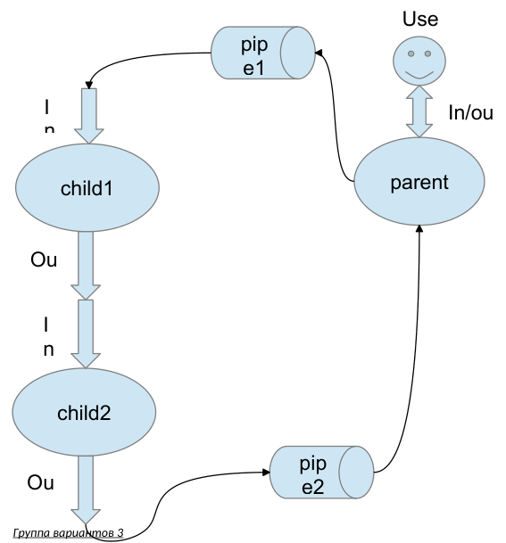
\includegraphics[width=0.55\textwidth]{process_cheme.png}
  \caption{Схема взаимодействия процессов}
  \label{fig:process-scheme}
\end{figure}


\section{Описание программы}

Программа состоит из трёх исходных файлов: \texttt{parent.c}, \texttt{child1.c} и \texttt{child2.c}. Файл \texttt{parent.c} содержит логику создания каналов и дочерних процессов, передачи пользовательского ввода и получения результата. \texttt{child1.c} отвечает за перевод символов в нижний регистр, \texttt{child2.c} --- за замену пробельных символов на \texttt{\_}.
Родительский процесс создаёт два дочерних процесса: child1 и child2. Для обмена данными между процессами создаются три неименованных канала: первый передаёт данные от parent к child1, второй - от child1 к child2, третий - от child2 обратно к parent.
